%--- Implementation
\begin{figure}[h!]
    \centering
    \caption{Effects of \emph{Plan Cuadrante} by Population Density, Poverty, and Socioeconomic Status}
    \label{fig:figure04_het}
    \begin{subfigure}[t]{0.49\textwidth}
        \centering
        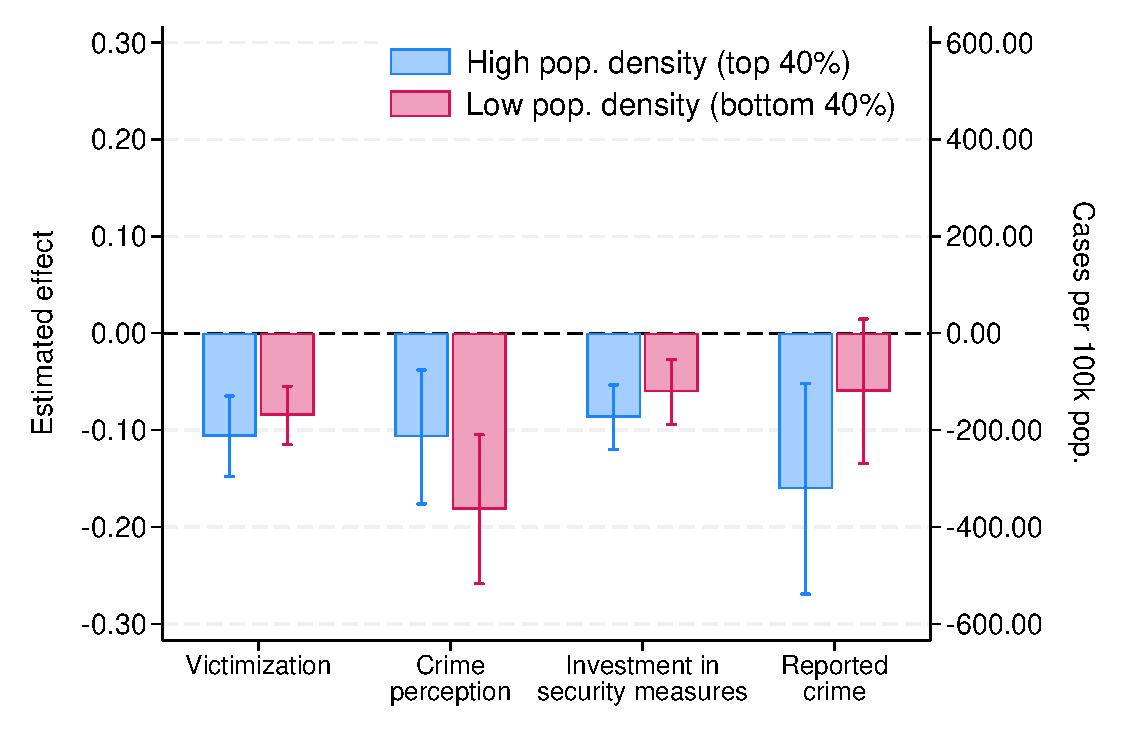
\includegraphics[width=\linewidth]{../manuscript/Graphs/results_het_density.pdf}
        \caption{By population density}
    \end{subfigure}\hfill
    \begin{subfigure}[t]{0.49\textwidth}
        \centering
        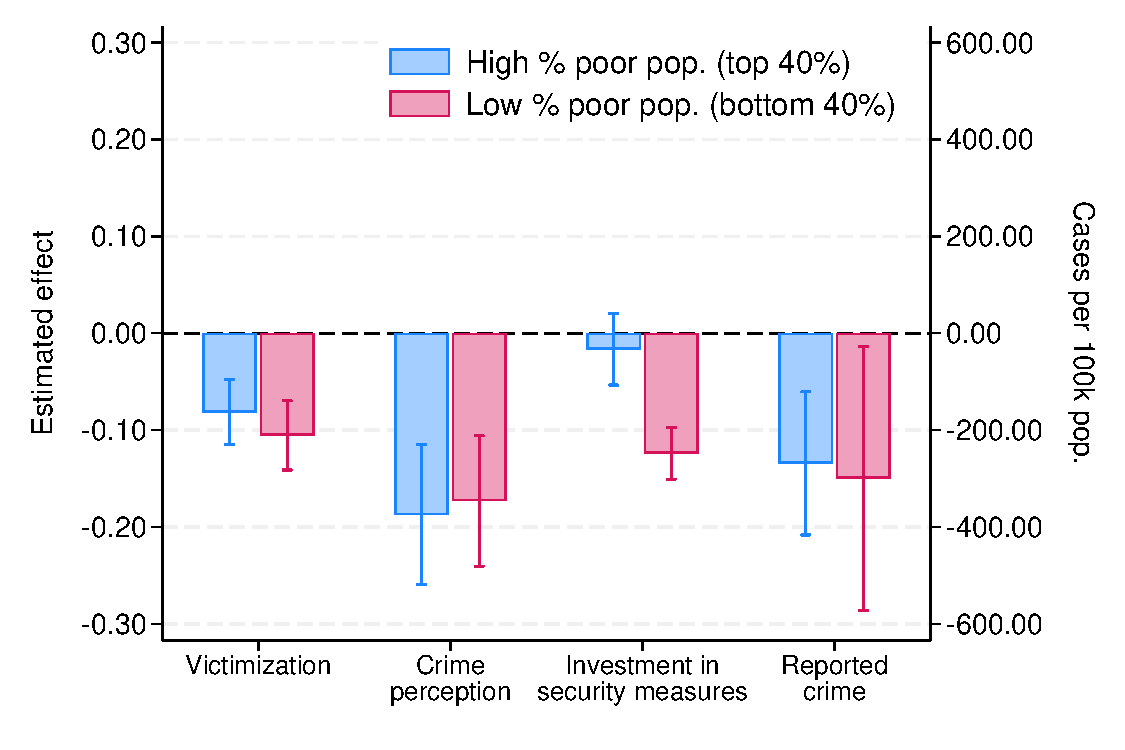
\includegraphics[width=\linewidth]{../manuscript/Graphs/results_het_poorpop.pdf}
        \caption{By population below poverty line}
    \end{subfigure}
    \\[8pt]
    \begin{subfigure}[t]{0.49\textwidth}
        \centering
        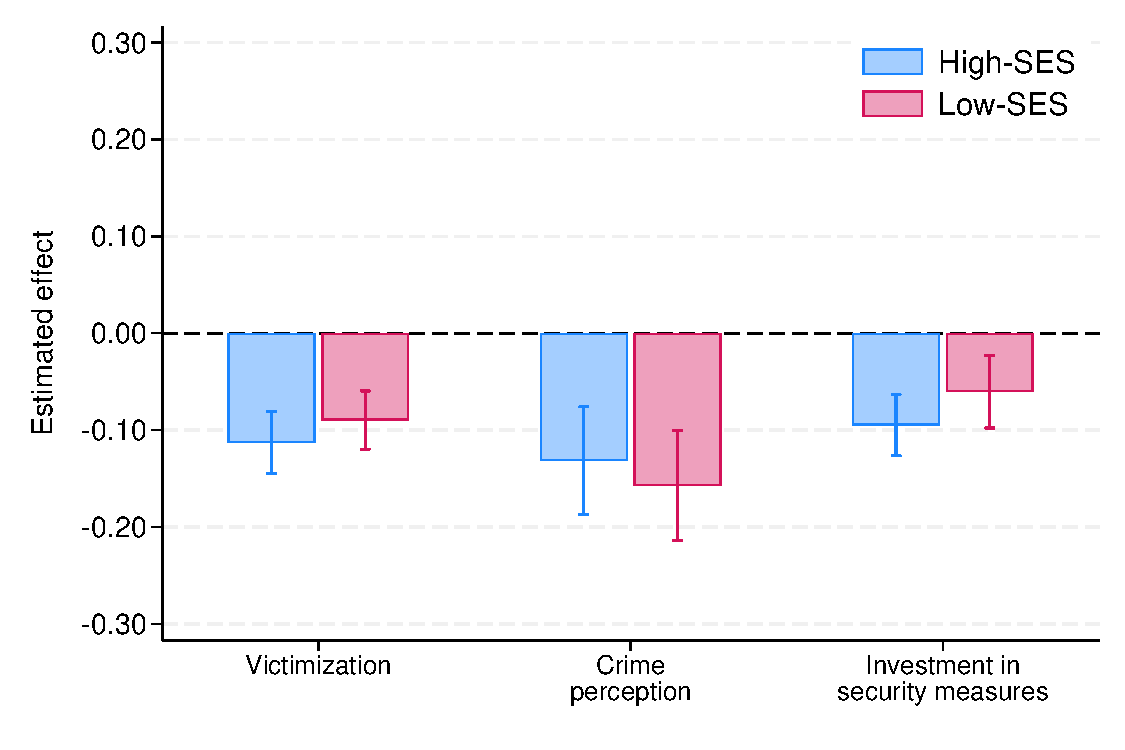
\includegraphics[width=\linewidth]{../manuscript/Graphs/results_het_SES.pdf}
        \caption{By household socioeconomic status}
    \end{subfigure}
    \\[10pt]
    \begin{minipage}{0.99\textwidth}
    \footnotesize Notes: This figure reports the heterogeneous effects of \emph{Plan Cuadrante} by population density (panel a), the proportion of poor people in the municipality (panel b), and household socioeconomic status (panel c). Each panel reports the effect on victimization, defined as the probability of household victimization in the last 12 months; crime perception, defined as the probability of perceiving an increase in crime; investment in security measures, defined as the probability of adopting security measures in the last twelve months; and reported crime, defined as the number of crimes reported to the police in the municipality per 100,000 inhabitants. Reported crime (administrative data, in cases per 100,000 inhabitants) is read on the right axis; all other outcomes, from the ENUSC survey (victimization, crime perception, and investment in security measures), are read on the left axis. Household socioeconomic status is only observed in the ENUSC, so panel (c) does not include reported crime. In panels (a) and (b), the bars compare municipalities in the two bottom quintiles (bottom 40\%) and in the two top quintiles (top 40\%) of the population density and poverty distributions, respectively. The average population density is 458 inhabitants per square kilometer in high-density municipalities and 29 in low-density municipalities; the average poverty rate is 28\% in high-poverty municipalities and 14\% in low-poverty municipalities. In panel (c), low-SES households include lower-class and lower-middle-class households, while high-SES households include upper-middle and upper-class households. The estimation is conducted using the difference-in-differences estimator for staggered treatment adoption developed in \citet{Callaway}. The graphs display the estimated coefficients and 95\% confidence intervals. Standard errors are clustered at the municipality level using the wild bootstrapping procedure.
    \end{minipage}
\end{figure}
